%% abtex2-modelo-relatorio-tecnico.tex, v-1.7.1 laurocesar
%% Copyright 2012-2013 by abnTeX2 group at http://abntex2.googlecode.com/ 
%%
%% This work may be distributed and/or modified under the
%% conditions of the LaTeX Project Public License, either version 1.3
%% of this license or (at your option) any later version.
%% The latest version of this license is in
%%   http://www.latex-project.org/lppl.txt
%% and version 1.3 or later is part of all distributions of LaTeX
%% version 2005/12/01 or later.
%%
%% This work has the LPPL maintenance status `maintained'.
%% 
%% The Current Maintainer of this work is the abnTeX2 team, led
%% by Lauro César Araujo. Further information are available on 
%% http://abntex2.googlecode.com/
%%
%% This work consists of the files abntex2-modelo-relatorio-tecnico.tex,
%% abntex2-modelo-include-comandos and abntex2-modelo-references.bib
%%

% ------------------------------------------------------------------------
% ------------------------------------------------------------------------
% abnTeX2: Modelo de Relatório Técnico/Acadêmico em conformidade com 
% ABNT NBR 10719:2011 Informação e documentação - Relatório técnico e/ou
% científico - Apresentação
% ------------------------------------------------------------------------ 
% ------------------------------------------------------------------------

% Alterado por Rodrigo Campiolo para apresentação de relatórios na disciplina
% de Redes de Computadores II do Bacharelado em Ciência da Computação da UTFPR-CM.


\documentclass[
	% -- opções da classe memoir --
	12pt,				% tamanho da fonte
	%openright,			% capítulos começam em pág ímpar (insere página vazia caso preciso)
	oneside,   	        % para impressão em verso e anverso use twoside. Oposto a oneside
	a4paper,			% tamanho do papel. 
	% -- opções da classe abntex2 --
	%chapter=TITLE,		% títulos de capítulos convertidos em letras maiúsculas
	%section=TITLE,		% títulos de seções convertidos em letras maiúsculas
	%subsection=TITLE,	% títulos de subseções convertidos em letras maiúsculas
	%subsubsection=TITLE,% títulos de subsubseções convertidos em letras maiúsculas
	% -- opções do pacote babel --
	english,			% idioma adicional para hifenização
	french,				% idioma adicional para hifenização
	spanish,			% idioma adicional para hifenização
	brazil,				% o último idioma é o principal do documento
	]{pacotes/abntex2}


% ---
% PACOTES
% ---

% ---
% Pacotes fundamentais 
% ---
\usepackage{cmap}				% Mapear caracteres especiais no PDF
\usepackage{lmodern}			% Usa a fonte Latin Modern
\usepackage[T1]{fontenc}		% Selecao de codigos de fonte.
\usepackage[utf8]{inputenc}		% Codificacao do documento (conversão automática dos acentos)
\usepackage{indentfirst}		% Indenta o primeiro parágrafo de cada seção.
\usepackage{color}				% Controle das cores
\usepackage{graphicx}			% Inclusão de gráficos
% ---

% ---
% Pacotes adicionais, usados no anexo do modelo de folha de identificação
% ---
\usepackage{multicol}
\usepackage{multirow}
% ---
	
% ---
% Pacotes adicionais, usados apenas no âmbito do Modelo Canônico do abnteX2
% ---
\usepackage{lipsum}				% para geração de dummy text
% ---

% ---
% Pacotes de citações
% ---
\usepackage[brazilian,hyperpageref]{backref}	 % Paginas com as citações na bibl
\usepackage[alf]{pacotes/abntex2cite}	% Citações padrão ABNT
\usepackage{comment}

% ---
% Meus pacotes
% ---
\usepackage{float}
\usepackage{array}
% ---

% --- 
% CONFIGURAÇÕES DE PACOTES
% --- 

% ---
% Configurações do pacote backref
% Usado sem a opção hyperpageref de backref
\renewcommand{\backrefpagesname}{Citado na(s) página(s):~}
% Texto padrão antes do número das páginas
\renewcommand{\backref}{}
% Define os textos da citação
\renewcommand*{\backrefalt}[4]{
	\ifcase #1 %
		Nenhuma citação no texto.%
	\or
		Citado na página #2.%
	\else
		Citado #1 vezes nas páginas #2.%
	\fi}%
% ---

% ---
% Informações de dados para CAPA e FOLHA DE ROSTO
% ---
\titulo{Simulação de Algoritmos de Escalonamento}
\autor{Hendrick Felipe Scheifer\\João Victor Briganti\\Luiz Gustavo Takeda}
\local{Campo Mourão}
\data{Novembro / 2024}
\instituicao{%
  Universidade Tecnológica Federal do Paraná -- UTFPR
  \par
  Departamento Acadêmico de Computação -- DACOM
  \par
  Bacharelado em Ciência da Computação -- BCC
}
\tipotrabalho{Relatório técnico}
% O preambulo deve conter o tipo do trabalho, o objetivo, 
% o nome da instituição e a área de concentração 
\preambulo{Relatório técnico de atividade prática solicitado pelo professor Rodrigo Campiolo na disciplina de Redes de Computadores II do Bacharelado em Ciência da Computação da Universidade Tecnológica Federal do Paraná.}
% ---

% ---
% Configurações de aparência do PDF final

% alterando o aspecto da cor azul
\definecolor{blue}{RGB}{41,5,195}

% informações do PDF
\makeatletter
\hypersetup{
     	%pagebackref=true,
		pdftitle={\@title}, 
		pdfauthor={\@author},
    	pdfsubject={\imprimirpreambulo},
	    pdfcreator={LaTeX with abnTeX2},
		pdfkeywords={abnt}{latex}{abntex}{abntex2}{relatório técnico}, 
		colorlinks=true,       		% false: boxed links; true: colored links
    	linkcolor=blue,          	% color of internal links
    	citecolor=blue,        		% color of links to bibliography
    	filecolor=magenta,      		% color of file links
		urlcolor=blue,
		bookmarksdepth=4
}
\makeatother
% --- 

% --- 
% Espaçamentos entre linhas e parágrafos 
% --- 

% O tamanho do parágrafo é dado por:
\setlength{\parindent}{1.3cm}

% Controle do espaçamento entre um parágrafo e outro:
\setlength{\parskip}{0.2cm}  % tente também \onelineskip

% ---
% compila o indice
% ---
\makeindex
% ---

% Omite a numeração de capítulos
\renewcommand*\thesection{\arabic{section}}



% ----
% Início do documento
% ----
\begin{document}

% Retira espaço extra obsoleto entre as frases.
\frenchspacing 

% ----------------------------------------------------------
% ELEMENTOS PRÉ-TEXTUAIS
% ----------------------------------------------------------
% \pretextual

% ---
% Capa
% ---
%\imprimircapa
% ---

% ---
% Folha de rosto
% (o * indica que haverá a ficha bibliográfica)
% ---
\imprimirfolhaderosto
% ---


% ---
% RESUMO
% ---

% resumo na língua vernácula (obrigatório)
\begin{resumo}
Este trabalho visa explorar os conceitos fundamentais sobre escalonamento de processos a partir da compreensão, simulação e análise de diferentes algoritmos de escalonamento. Para realizar esta prática, os diferentes algoritmos de escalonamento foram testados com o simulador OS Sim para a análise de tempos e métricas de execução, permitindo avaliar o impacto de diferentes estratégias no escalonamento de processos. 
 \vspace{\onelineskip}
    
 \noindent
 \textbf{Palavras-chave}: Processos; Escalonamento; Sistema Operacional.
\end{resumo}
% ---

% ---
% inserir lista de ilustrações
% ---
%\pdfbookmark[0]{\listfigurename}{lof}
%\listoffigures*
%\cleardoublepage
% ---

% ---
% inserir lista de tabelas
% ---
%\pdfbookmark[0]{\listtablename}{lot}
%\listoftables*
%\cleardoublepage
% ---

% ---
% inserir lista de abreviaturas e siglas
% ---
%\begin{siglas}
%  \item[IP] Internet Protocol
%  \item[TCP] Transmission Control Protocol
%  \item[UDP] User Datagram Protocol
%\end{siglas}
% ---

% ---
% inserir o sumario
% ---
\pdfbookmark[0]{\contentsname}{toc}
\tableofcontents*
\cleardoublepage
% ---

% ----------------------------------------------------------
% ELEMENTOS TEXTUAIS
% ----------------------------------------------------------
\textual

\makeatletter
\renewcommand{\chapter}{\@gobbletwo}
\makeatother

\section{Introdução}
\label{sec:introducao}
Com a grande quantidade de processos executados em um computador, é válida a preocupação com a gerência do processador, ou seja, com o gerenciamento dos processos que estão sendo realizado pelo processador durante seu tempo de uso. Este gerenciamento é chamado escalonamento de processos, e é extremamente importante em sistemas operacionais multiprogramados, onde diversas aplicações disputam pelo uso do processador ao mesmo tempo. Sempre que mais de um processo estão no estado de pronto, o sistema operacional deve realizar uma escolha sobre o processo que assumirá o processador a seguir. Esta escolha pode ser realizada de diferentes formas, e os algoritmos implementados para isso são chamados algoritmos de escalonamento~\cite{tanenbaum2016}.

\section{Objetivos}
\label{sec:objetivos}
Os objetivos deste trabalho são compreender diferentes algoritmos básicos de escalonamento com o auxílio de um simulador, e analisar o comportamento e desempenho dos diferentes algoritmos de escalonamento.

\section{Fundamentação}
\label{sec:fundamentacao}
Para compreender o escalonamento de processos, é necessário compreender que processos possuem duas naturezas distintas que definem seu comportamento, existem processos que passam a maior parte do tempo dependendo do processador para sua execução, estes são chamados de processos orientados a processador (\textit{CPU Bound}), e, por outro lado, existem processos que dependem mais de entradas e saídas, dependendo menos do processador, estes são os processos orientados a Entrada/Saída (\textit{I/O Bound})~\cite{tanenbaum2016}.

Outro conceito importante a levar-se em consideração é o conceito de sistemas preemptivos e cooperativos. Sistemas cooperativos são mais simples de controlar, pois cada tarefa que assumir o processador, irá permanecer em execução até o seu término, para que, apenas após ser terminada, outro processo assuma o processador. Em sistemas preemptivos, cada processo que assume o processador corre o risco de ser suspenso de sua execução em algumas situações a variar conforme o algoritmo de escalonamento utilizado, isso pode acontecer quando o processo possui um \textit{quantum} de tempo no processador e seu tempo chega ao fim ou quando um processo que possui uma prioridade maior está no estado de pronto e devido a sua prioridade, assumirá o processador~\cite{maziero2019}.

Os algoritmos de escalonamento utilizam um critério para definir qual processo deve assumir o processador, além de levar em consideração a possível existência de mais de um núcleo de processamento, o que garante a execução simultânea de mais de um processo. A seção 5 detalha e realiza medições sobre diferentes algoritmos de escalonamento.

\section{Materiais}
\label{sec:materiais}

Simulador OS Sim na versão 1.2.

\section{Procedimentos e Resultados}
\label{sec:procedimentos}

O simulador OS Sim foi utilizado para analisar tempos de execução e outras métricas, avaliando o impacto de diferentes estratégias de escalonamento de processos. Esse estudo permitiu observar como cada algoritmo distribui as tarefas, influenciando a eficiência e o desempenho do sistema. Vale destacar que alguns valores fornecidos pelo simulador, especialmente os relacionados à porcentagem de uso da CPU, apresentaram inconsistências. Por essa razão, alguns desses dados precisaram ser recalculados.

\subsection{FCFS (\textit{First-Come, First-Served})}
\label{subsec:fcfs}

O primeiro algoritmo analisado foi o FCFS, um dos algoritmos de escalonamento mais simples, ele funciona da seguinte maneira o processo a chegar ao estado de pronto é o primeiro a ser atendido, o segundo a chegar é o segundo a ser atendido, o terceiro a chegar é o terceiro a ser atendido e assim sucessivamente~\cite{maziero2019}. 

\subsubsection{FCFS \textit{First-Come, First-Served} Monoprogramação}
\label{subsubsec:mono_fcfs}

A primeira versão simulada deste algoritmo se deu em um ambiente de monoprogramação, na prática, isso significa que apenas um programa pode estar na memória e executando na CPU ao mesmo tempo, dessa forma processos que realizam chamadas de E/S (Entrada/Saída) não podem ser colocados em estado de bloqueado, pois não há como trazer outro processo a memória para executar de maneira concorrente ao processo em execução. Desse modo, neste ambiente o programa que entrar em execução assumirá o processador até o final, mesmo que entre em estado de bloqueado~\cite{tanenbaum2016}.

A Figura~\ref{fig:fcfs_mono} apresenta o diagrama de Grant com o período de execução de cada processo. Os períodos em azul simbolizam a execução na CPU enquanto os amarelos são períodos de execução de E/S.

\begin{figure}[H]
  \centering
  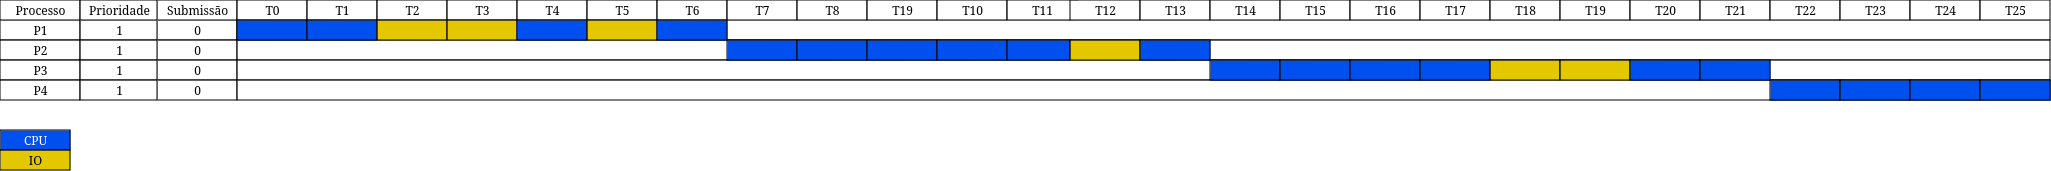
\includegraphics[scale=0.20]{figuras/ex1/fcfs_mono.png}
  \caption{Diagrama de Grant do algoritmo FCFS em um ambiente monoprogramado.}
  \label{fig:fcfs_mono}
\end{figure}

A Figura~\ref{fig:table_fcfs_mono} apresenta uma tabela com informações de execução deste algoritmo. O tempo de criação do processo e o seu tempo de execução aumentaram conforme a posição do processo na fila, o fato de alguns processos não estarem utilizando a CPU em  alguns momentos e mesmo assim consumindo seu tempo, acaba degradando bastante a execução dos processos de maneira geral.

\begin{figure}[H]
  \centering
  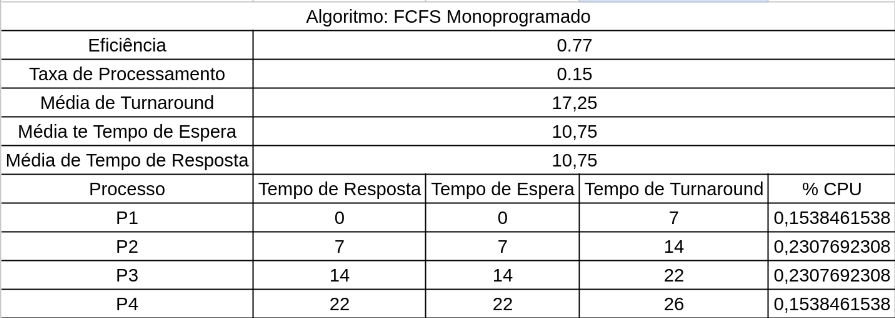
\includegraphics[scale=0.5]{figuras/ex1/table_fcfs_mono.png}
  \caption{Tabela com informações de execução do FCFS em um ambiente de monoprogramação.}
  \label{fig:table_fcfs_mono}
\end{figure}

\subsubsection{FCFS \textit{First-Come, First-Served} Multiprogramação}
\label{subsubsec:multi_fcfs}

Nesta segunda versão o algoritmo está em maneira multiprogramada, o que significa que mais de um programa pode estar na memória, o que vai permitir uma execução concorrente entre os processos. Desse modo, processos que realizam chamadas de E/S podem ser colocados no estado de bloqueado e passam sua vez para que outro processo faça uso da CPU. Neste caso, processos que perdem sua vez na CPU, são colocados ao final da fila. 

A Figura~\ref{fig:fcfs_multi} apresenta o diagrama de Grant que ilustra os períodos de execução de cada processo.

\begin{figure}[H]
  \centering
  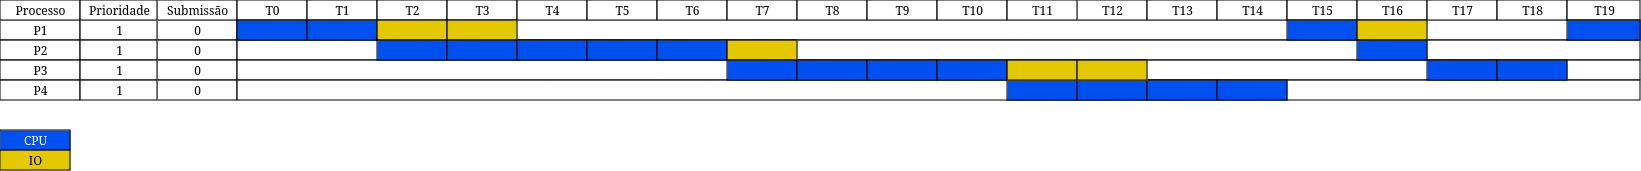
\includegraphics[scale=0.20]{figuras/ex1/fcfs_multi.png}
  \caption{Diagrama de Grant do algoritmo FCFS em um ambiente multiprogramado.}
  \label{fig:fcfs_multi}
\end{figure}

A Figura~\ref{fig:table_fcfs_mono} apresenta uma tabela com informações de execução deste algoritmo. É possível perceber que este algoritmo, diferente da versão anterior~\ref{subsubsec:mono_fcfs}, faz um uso mais eficiente da CPU, pois em nenhum momento ela fica ociosa, porém, nesta versão do algoritmo processos que realizam E/S acabam sendo penalizados, pois são colocados ao final da fila.

\begin{figure}[H]
  \centering
  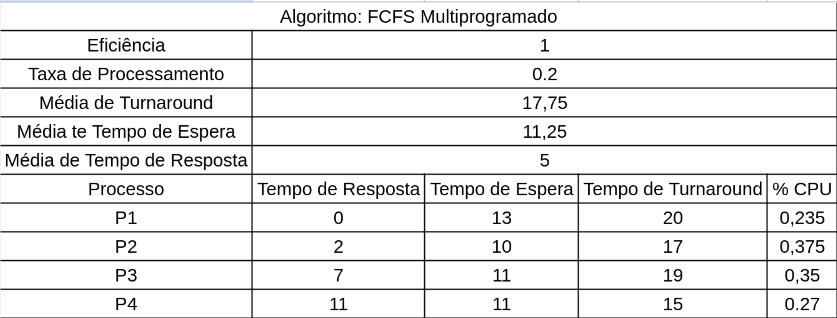
\includegraphics[scale=0.5]{figuras/ex1/table_fcfs_multi.png}
  \caption{Tabela com informações de execução do algoritmo FCFS em um ambiente de multiprogramação.}
  \label{fig:table_fcfs_multi}
\end{figure}

\subsection{Prioridade}
\label{subsec:prio}

O segundo algoritmo analisado foi o de prioridades, existem diferentes formas de se implementar esse algoritmo, no caso a escolhida pelo simulador é a de prioridades fixas. O algoritmo de prioridades fixas trabalha com a ideia de que cada processo possui uma prioridade associada, que não se altera ao longo da execução. Nesta sessão são analisadas duas variantes desse algoritmo, sua versão preemptiva e sua versão não preemptiva~\cite{maziero2019}.

\subsubsection{Prioridade Estática Não Preemptiva}
\label{subsubsec:prio_sem_preemp}

A preempção dentro de Sistemas Operacionais, está relacionada a retirar um processo que está atualmente executando da CPU para dar espaço para que outro processo execute. Quando se trata de um algoritmo de prioridade não preemptivo, isso significa que a partir do momento que um processo começou a ser executado, ele não perderá o controle da CPU, a menos que ele realize uma operação de E/S ou finalize sua execução, seja ela uma finalização normal ou devido a um erro~\cite{maziero2019}.

Neste algoritmo de prioridade estática não preemptiva, o que ocorre é que o escalonador ao se deparar com dois processos na fila de aptos, irá escolher aquele com maior prioridade. A Figura~\ref{fig:prio_sem_preemp} apresenta um diagrama de Grant que ilustra a execução deste algoritmo.

\begin{figure}[H]
  \centering
  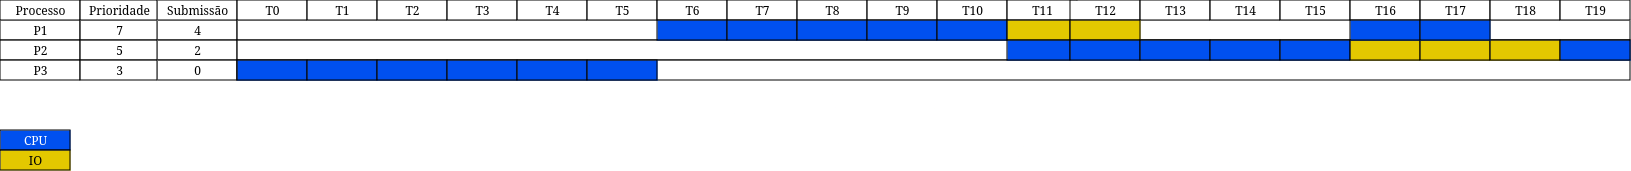
\includegraphics[scale=0.20]{figuras/ex2/prio_sem_preemp.png}
  \caption{Diagrama de Grant do algoritmo de Prioridade Estática Sem Preempção.}
  \label{fig:prio_sem_preemp}
\end{figure}

A Figura~\ref{fig:table_prio_sem_preemp} mostra uma tabela com algumas informações relacionadas a execução deste algoritmo. É possível perceber que está execução não atingiu 100\% de eficiência. Um dos grandes problemas observado dessa falta de preempção é que processos mais prioritários, em dados momentos, precisam esperar processos menos prioritários terminarem sua execução, o que se torna problemático se considerarmos que a proposta do algoritmo é que processos mais prioritários sejam atendidos primeiro.

\begin{figure}[H]
  \centering
  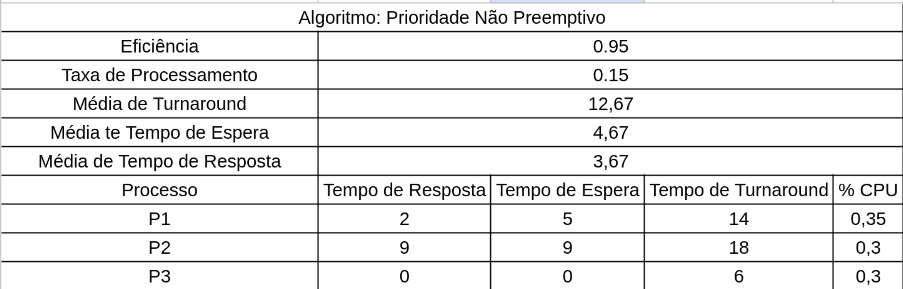
\includegraphics[scale=0.5]{figuras/ex2/table_prio_sem_preemp.png}
  \caption{Tabela com informações de execução do algoritmo de Prioridade Estática Sem Preempção.}
  \label{fig:table_prio_sem_preemp}
\end{figure}

\subsubsection{Prioridade Estática Preemptiva}
\label{subsubsec:prio_preemp}

Nesta versão do algoritmo temos o processo de preempção, onde um processo em andamento dá lugar a outro processo de maior prioridade executar. Sempre que um processo de maior prioridade do que o que está atualmente executando chegar na fila de aptos, uma preempção ocorre.

 A Figura~\ref{fig:prio_preemp} apresenta um diagrama de Grant que ilustra a execução deste algoritmo.

\begin{figure}[H]
  \centering
  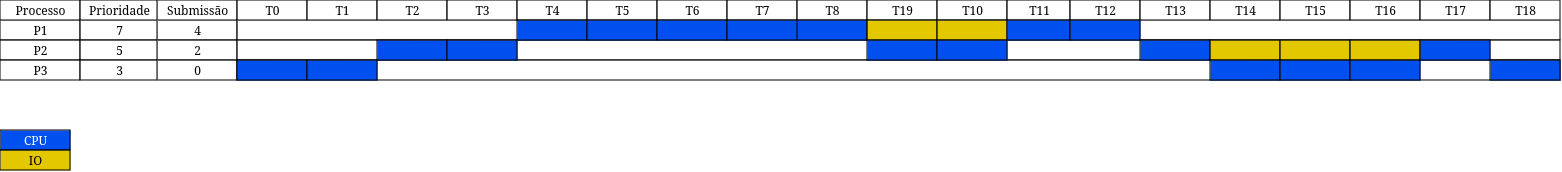
\includegraphics[scale=0.20]{figuras/ex2/prio_preemp.png}
  \caption{Diagrama de Grant do algoritmo de Prioridade Estática Preemptiva.}
  \label{fig:prio_preemp}
\end{figure}

A Figura~\ref{fig:table_prio_sem_preemp} apresenta uma tabela com informações sobre a execução desse algoritmo. Uma de suas vantagens é o menor tempo de resposta, pois um processo de alta prioridade é imediatamente colocado em execução assim que chega à fila de aptos. Isso reduz o tempo de resposta médio em comparação com a versão não preemptiva do algoritmo. No entanto, essa abordagem pode causar inanição: se processos mais prioritários continuarem chegando, eles sempre terão preferência, deixando processos de menor prioridade em espera por tempo indeterminado.

\begin{figure}[H]
  \centering
  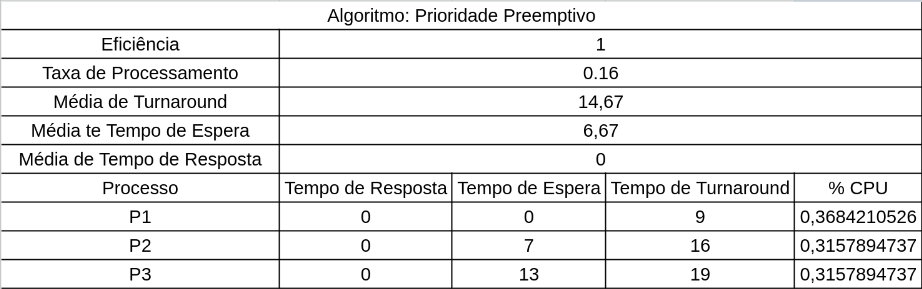
\includegraphics[scale=0.5]{figuras/ex2/table_prio_preemp.png}
  \caption{Tabela com informações de execução do algoritmo de Prioridade Estática Preemptiva.}
  \label{fig:table_prio_preemp}
\end{figure}

\subsection{Comparação Entre Algoritmos}
\label{subsec:algoritmos}

Para realizar a comparação entre os algoritmos foram usados 5 algoritmos diferentes, sendo eles~\cite{maziero2019}:

\begin{itemize}
  \item FCFS: Neste algoritmo o primeiro processo a chegar e o primeiro a ser atendido.
  \item SJF (\textit{Shortest Job First}): Algoritmo onde os processos com menos tempo de execução são executados primeiro. Foi testado sua versão com e sem preempção.
  \item Prioridade: Algoritmo de prioridade estático, onde o processo com maior prioridade na fila de aptos é escolhido para ser executado. Foi testado sua versão com e sem preempção.
  \item \textit{Round-Robin}: Neste algoritmo cada processo recebe uma fatia do tempo de execução, também chamada de \textit{quantum}, ao final deste período o processo dá espaço para que outro execute.
\end{itemize}

A simulação foi realizada com 4 processos, a configuração de cada processo pode ser observada na Tabela~\ref{table:processos}.

\begin{table}[H]
\centering
\caption{Informações de execução de cada processo}
\label{table:processos}
\footnotesize
\begin{tabular}{l|c|c|l}
\toprule
\textbf{Processo} & \textbf{Tempo de Submissão} & \textbf{Prioridade} & \textbf{\textit{Burst} (Duração e Tipo)} \\ 
\midrule
\textbf{P1} & 0  & 4 & 1 CPU + 1 E/S + 1 CPU + 1 E/S + 1 CPU \\
\textbf{P2} & 0  & 2 & 3 CPU + 1 E/S + 3 CPU \\
\textbf{P3} & 3  & 6 & 4 CPU + 4 E/S + 2 CPU \\
\textbf{P4} & 6  & 3 & 4 CPU \\
\bottomrule
\end{tabular}
\end{table}

\subsubsection{Execução FCFS Multiprogramado}
\label{subsubsec:fcfs_multi}

A Figura~\ref{fig:ex3/diagrama/fcfs_multi} apresenta um diagrama de Grant que exemplifica a execução dos processos pelo algoritmo FCFS. A Figura~\ref{fig:ex3/tabela/fcfs_multi} apresenta uma tabela com informações detalhadas sobre a execução dos processos. Os problemas que encontramos neste algoritmo são os mesmos já citados na seção~\ref{subsubsec:fcfs_multi}.

\begin{figure}[H]
  \centering
  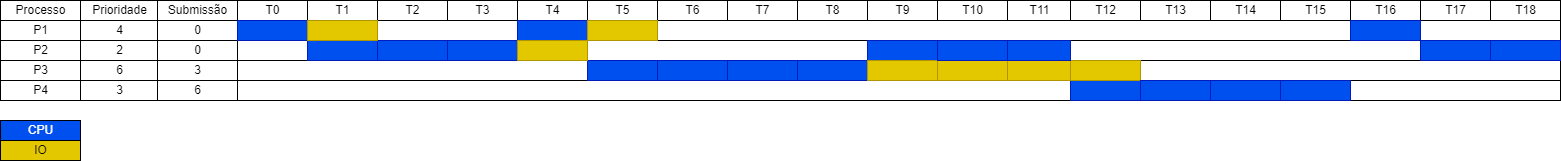
\includegraphics[scale=0.20]{figuras/ex3/diagrama/fcfs_multi.png}
  \caption{Diagrama de Grant do algoritmo FCFS em um ambiente multiprogramado.}
  \label{fig:ex3/diagrama/fcfs_multi}
\end{figure}

\begin{figure}[H]
  \centering
  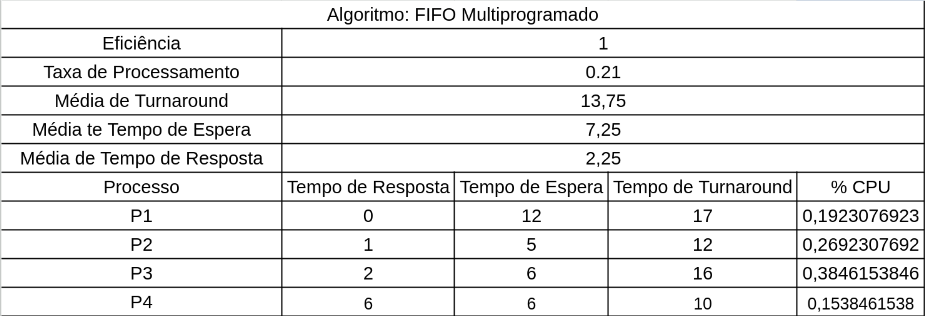
\includegraphics[scale=0.5]{figuras/ex3/tabela/fcfs_multi.png}
  \caption{Tabela com informações de execução do FCFS em um ambiente multiprogramado.}
  \label{fig:ex3/tabela/fcfs_multi}
\end{figure}


\subsubsection{Execução Prioridade Estática Não Preemptiva}
\label{subsubsec:prio_sem_preemp}

A Figura~\ref{fig:ex3/diagrama/prio_sem_preemp} apresenta um diagrama de Grant que exemplifica a execução dos processos pelo algoritmo de Prioridade Estático Não Preemptivo. A Figura~\ref{fig:ex3/tabela/prio_sem_preemp} apresenta uma tabela com informações detalhadas sobre a execução dos processos. 

\begin{figure}[H]
  \centering
  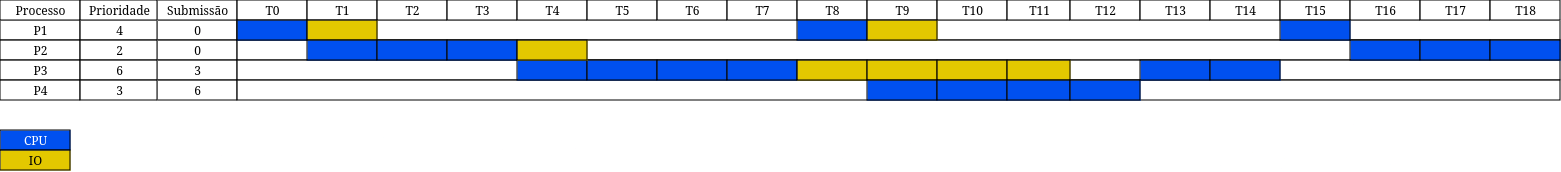
\includegraphics[scale=0.20]{figuras/ex3/diagrama/prio_sem_preemp.png}
  \caption{Diagrama de Grant do algoritmo Prioridade Estático Não Preemptivo.}
  \label{fig:ex3/diagrama/prio_sem_preemp}
\end{figure}

\begin{figure}[H]
  \centering
  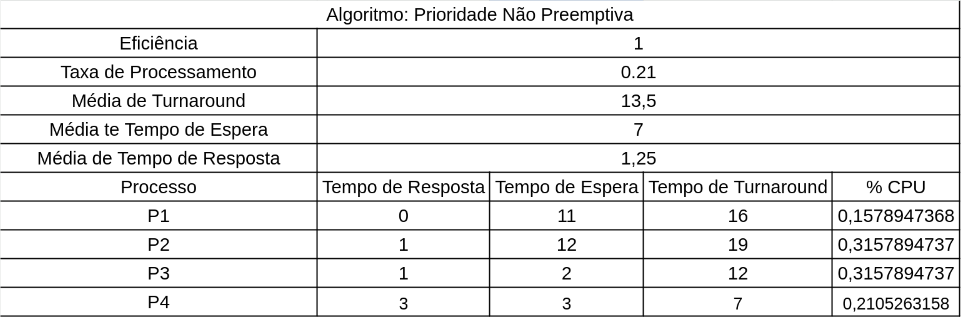
\includegraphics[scale=0.5]{figuras/ex3/tabela/prio_sem_preemp.png}
  \caption{Tabela com informações de execução do algoritmo Prioridade Estático Não Preemptivo.}
  \label{fig:ex3/tabela/prio_sem_preemp}
\end{figure}

\subsubsection{Execução Prioridade Estática Preemptiva}
\label{subsubsec:prio_preemp}

A Figura~\ref{fig:ex3/diagrama/prio_preemp} apresenta um diagrama de Grant que exemplifica a execução dos processos pelo algoritmo de Prioridade Estático Preemptivo. A Figura~\ref{fig:ex3/tabela/prio_preemp} apresenta uma tabela com informações detalhadas sobre a execução dos processos. 

\begin{figure}[H]
  \centering
  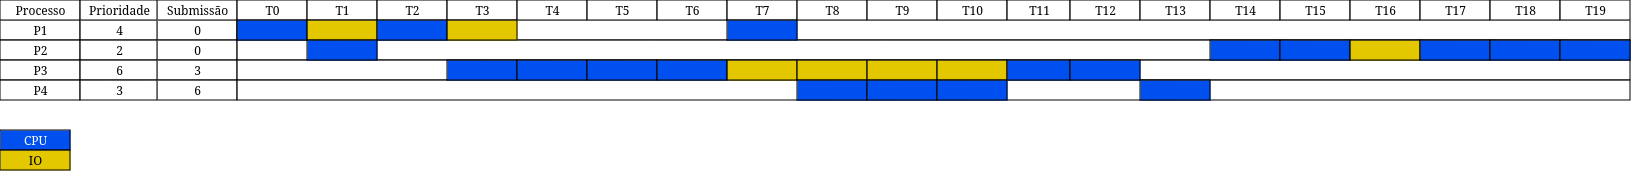
\includegraphics[scale=0.20]{figuras/ex3/diagrama/prio_preemp.png}
  \caption{Diagrama de Grant do algoritmo Prioridade Estático Preemptivo.}
  \label{fig:ex3/diagrama/prio_preemp}
\end{figure}

\begin{figure}[H]
  \centering
  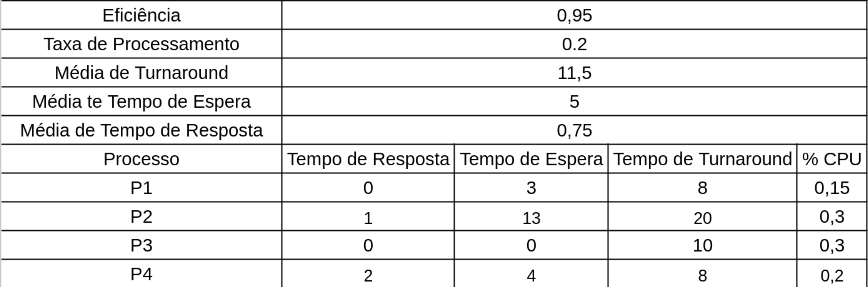
\includegraphics[scale=0.5]{figuras/ex3/tabela/prio_preemp.png}
  \caption{Tabela com informações de execução do algoritmo Prioridade Estático Preemptivo.}
  \label{fig:ex3/tabela/prio_preemp}
\end{figure}

\subsubsection{Execução SJF Não Preemptiva}
\label{subsubsec:sjf_sem_preemp}

A Figura~\ref{fig:ex3/diagrama/sjf_sem_preemp} apresenta um diagrama de Grant que exemplifica a execução dos processos pelo algoritmo de SJF Não Preemptivo. A Figura~\ref{fig:ex3/tabela/prio_preemp} apresenta uma tabela com informações detalhadas sobre a execução dos processos. 

\begin{figure}[H]
  \centering
  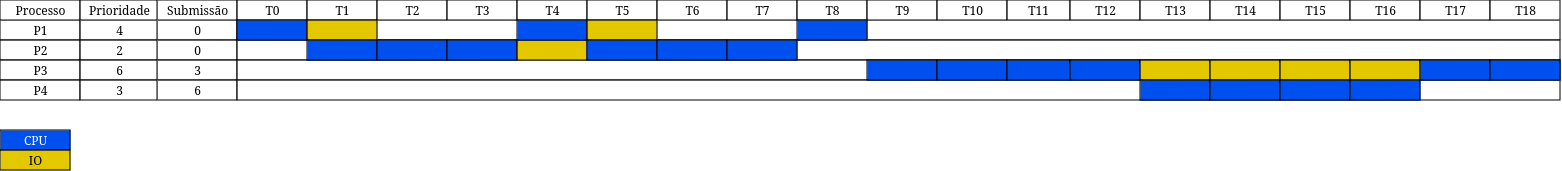
\includegraphics[scale=0.20]{figuras/ex3/diagrama/sjf_sem_preemp.png}
  \caption{Diagrama de Grant do algoritmo SJF Não Preemptivo.}
  \label{fig:ex3/diagrama/sjf_sem_preemp}
\end{figure}

\begin{figure}[H]
  \centering
  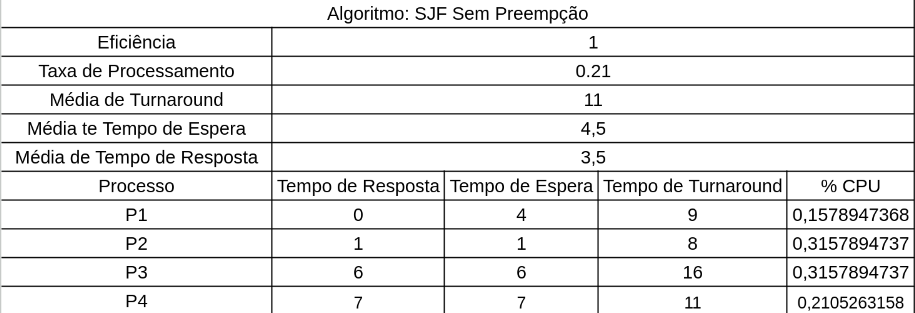
\includegraphics[scale=0.5]{figuras/ex3/tabela/sjf_sem_preemp.png}
  \caption{Tabela com informações de execução do algoritmo SJF Não Preemptivo.}
  \label{fig:ex3/tabela/sjf_sem_preemp}
\end{figure}

\subsubsection{Execução SJF Preemptiva}
\label{subsubsec:sjf_preemp}

A Figura~\ref{fig:ex3/diagrama/sjf_sem_preemp} apresenta um diagrama de Grant que exemplifica a execução dos processos pelo algoritmo de SJF Preemptivo. A Figura~\ref{fig:ex3/tabela/prio_preemp} apresenta uma tabela com informações detalhadas sobre a execução dos processos.

\begin{figure}[H]
  \centering
  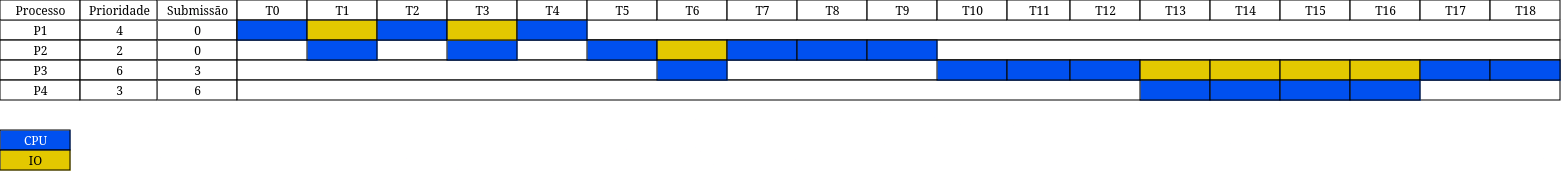
\includegraphics[scale=0.20]{figuras/ex3/diagrama/sjf_preemp.png}
  \caption{Diagrama de Grant do algoritmo SJF Preemptivo.}
  \label{fig:ex3/diagrama/sjf_sem_preemp}
\end{figure}

\begin{figure}[H]
  \centering
  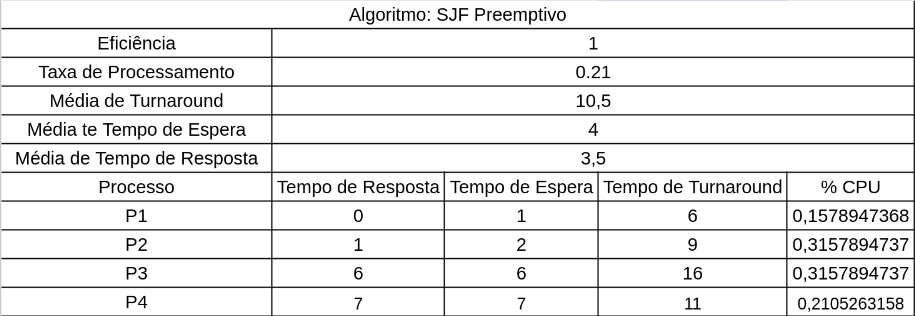
\includegraphics[scale=0.5]{figuras/ex3/tabela/sjf_preemp.png}
  \caption{Tabela com informações de execução do algoritmo SJF Preemptivo.}
  \label{fig:ex3/tabela/sjf_preemp}
\end{figure}

\subsubsection{Execução \textit{Round-Robin} Preemptiva}
\label{subsubsec:rr}

A Figura~\ref{fig:ex3/diagrama/sjf_sem_preemp} apresenta um diagrama de Grant que exemplifica a execução dos processos pelo algoritmo de \textit{Round-Robin}. A Figura~\ref{fig:ex3/tabela/rr} apresenta uma tabela com informações detalhadas sobre a execução dos processos. 

\begin{figure}[H]
  \centering
  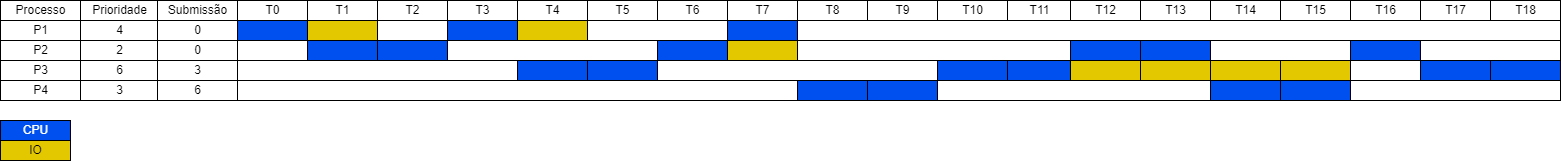
\includegraphics[scale=0.20]{figuras/ex3/diagrama/rr.png}
  \caption{Diagrama de Grant do algoritmo \textit{Round-Robin}.}
  \label{fig:ex3/diagrama/rr}
\end{figure}

\begin{figure}[H]
  \centering
  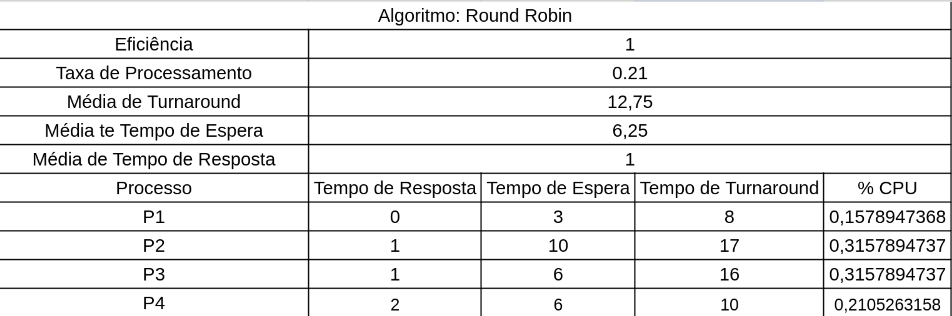
\includegraphics[scale=0.5]{figuras/ex3/tabela/rr.png}
  \caption{Tabela com informações de execução do algoritmo \textit{Round-Robin}.}
  \label{fig:ex3/tabela/rr}
\end{figure}

\subsubsection{Gráfico de Comparação}
\label{subsubsec:grafico}

A Figura~\ref{fig:media_tempo} apresenta um gráfico comparando os tempos médios de execução de cada algoritmo.

Os algoritmos de prioridade, tanto na versão preemptiva quanto na não preemptiva, apresentaram bons resultados em termos de tempo médio de resposta. Isso ocorreu porque processos de maior prioridade foram atendidos imediatamente após serem inseridos na fila. No entanto, se processos de menor prioridade forem adicionados posteriormente, seus tempos de resposta podem aumentar, pois serão preteridos em favor dos mais prioritários. Após os algoritmos de prioridade, o \textit{Round-Robin} obteve o segundo melhor tempo médio de resposta, o que era esperado devido à sua distribuição equitativa do tempo de execução por \textit{quantum}. Por fim, o algoritmo FCFS, que executa os processos na ordem de chegada, teve o pior desempenho, como esperado, já que ele executa os processos até o final, o que pode atrasar o tempo de resposta.

Quanto ao tempo médio de espera, o algoritmo SJF se destacou, pois prioriza processos mais curtos, permitindo que a fila avance mais rapidamente e reduzindo o tempo médio de espera. Em contraste, o FCFS apresentou a maior média de tempo de espera entre os algoritmos avaliados.

No que se refere ao tempo médio de \textit{turnaround}, não houve grandes variações, embora o SJF tenha mostrado um desempenho ligeiramente superior por priorizar processos que requerem menos tempo de CPU, acelerando sua execução.

De forma geral, os algoritmos SJF mantiveram um desempenho consistente, permanecendo próximos à média nas métricas de tempo. A escolha do algoritmo ideal depende das necessidades específicas da aplicação, levando em consideração as vantagens de cada abordagem no contexto de prioridades e requisitos de tempo.

\begin{figure}[H]
  \centering
  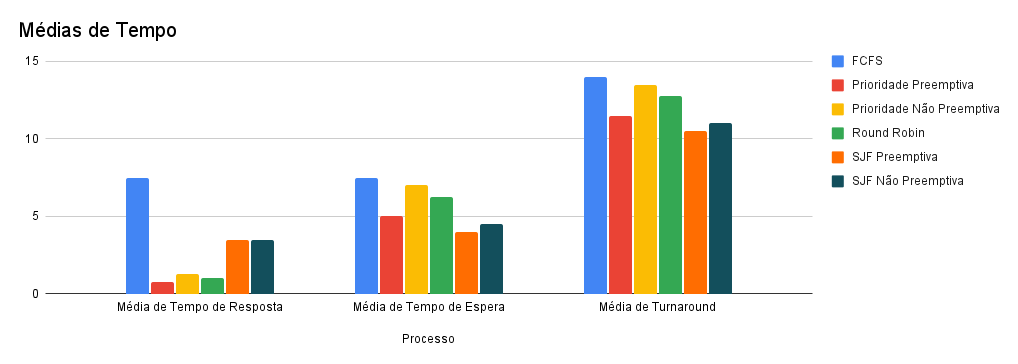
\includegraphics[scale=0.5]{figuras/ex3/grafico/media_tempo.png}
  \caption{Gráfico de comparação dos tempos médios de todos algoritmos.}
  \label{fig:media_tempo}
\end{figure}

\section{Conclusões}
\label{sec:conclusoes}
A análise e simulação de diferentes algoritmos de escalonamento de processos permitiram observar de que forma cada abordagem afeta o desempenho e a eficiência do sistema operacional. Cada algoritmo apresenta vantagens e desvantagens específicas, especialmente no que diz respeito a questões como tempo de resposta, utilização da CPU e eficiência. A comparação entre essas abordagens proporcionou uma visão detalhada de seus efeitos no desempenho global, auxiliando na escolha do algoritmo mais adequado conforme as necessidades específicas do sistema e das aplicações em execução.

% ----------------------------------------------------------
% ELEMENTOS PÓS-TEXTUAIS
% ----------------------------------------------------------
\postextual
% ----------------------------------------------------------
% Referências bibliográficas
% ----------------------------------------------------------
\renewcommand{\bibsection}{%
\section{\bibname}
\bibmark
%\ifnobibintoc\else
%\phantomsection
%\addcontentsline{toc}{section}{\bibname}
%\fi
\prebibhook}

\bibliography{abntex2-modelo-references}

\end{document}
